
%%%%%%%%%%%%%%%%%%%%%%%%%%%%%%%%%%%%%%
% Multiplicative domain poster
% Created by Nathaniel Johnston
% August 2009
% http://www.nathanieljohnston.com/index.php/2009/08/latex-poster-template/
%%%%%%%%%%%%%%%%%%%%%%%%%%%%%%%%%%%%%%

\documentclass[final,xcolor=pdftex,dvipsnames,table]{beamer}
\usepackage[scale=1.24]{beamerposter}
\usepackage{graphicx}			% allows us to import images
\usepackage{xcolor}
\usepackage{subfig}
\usepackage{framed}
\usepackage{general}
\usepackage{tikz-cd, fontenc}

%%%% OUR COMMANDS %%%%
\newcommand{\define}[1]{\textbf{#1}} % For all defined terms use this command
\newcommand{\mycomment}[1]{}

%-----------------------------------------------------------
% Define the column width and poster size
% To set effective sepwid, onecolwid and twocolwid values, 
%  first choose how many columns you want and how much 
%  separation you want between columns
% The separation I chose is 0.024 and I want 4 columns
% Then set onecolwid to be (1-(4+1)*0.024)/4 = 0.22
% Set twocolwid to be 2*onecolwid + sepwid = 0.464
%-----------------------------------------------------------

\newlength{\sepwid}
\newlength{\onecolwid}
\newlength{\twocolwid}
\setlength{\paperwidth}{48in}
\setlength{\paperheight}{36in}
\setlength{\sepwid}{0.024\paperwidth}
\setlength{\onecolwid}{0.22\paperwidth}%{0.30\paperwidth}
\setlength{\topmargin}{-0.5in}
\usetheme{confposter}

%-----------------------------------------------------------
% Define colours (see beamerthemeconfposter.sty to change these colour definitions)
%-----------------------------------------------------------

\setbeamercolor{block title}{fg=NavyBlue,bg=white}
%\setbeamercolor{block title}{fg=ngreen,bg=white}
%\setbeamercolor{block title}{fg=red,bg=white}
\setbeamercolor{block body}{fg=black,bg=white}
\setbeamercolor{block alerted title}{fg=white,bg=NavyBlue}
\setbeamercolor{block alerted body}{fg=black,bg=NavyBlue!10}

%----------------------------------------------------------------------------------------------------------------
% Name and authors of poster/paper/research
%----------------------------------------------------------------------------------------------------------------

\title{Spheres of Planes in Generalized Quaternions}
\author{% Alphabetical order
    Ian Gallagher,
    Andy Haase,
    Bailey Wickham, 
    Dr. Eric Brussel}
\institute{Department of Mathematics, California Polytechnic State University, San Luis Obispo}


%-----------------------------------------------------------
% Start the poster itself
%-----------------------------------------------------------
% The \rmfamily command is used frequently throughout the 
%  poster to force a serif font to be used for the body text
% Serif font is better for small text, sans-serif font is better for 
%  headers (for readability reasons)
%-----------------------------------------------------------
\usepackage{exscale}
\begin{document}
\begin{frame}[fragile]

%---- Cal Poly seal placed using tikz ----------------------------------%
\tikz [remember picture,overlay] 
	\node at ([yshift=-2in, xshift=4in]current page.north west) 
	{
\includegraphics[width=3in]{Paper-Poster/CalPolyLogo.png}};
\tikz [remember picture,overlay] 
	\node at ([yshift=-2in, xshift=-4in]current page.north east) 
	{
\includegraphics[width=3in]{Paper-Poster/CalPolyLogo.png}};
	
%\includegraphics[scale=2]{ImagesForPoster/SanLuisObispoSeal}

\begin{columns}[t]	   % the [t] option aligns the column's content at the top
\begin{column}{\sepwid}\end{column}	% empty spacer column
%---- COLUMN 1 ---------------------------------------------------------%
\begin{column}{\onecolwid}
%-------- BLOCK --------------------------------------------------------%
\begin{alertblock}{Abstract}
\rmfamily{% Content goes in \rmfamily{...}
A great discovery of Hamilton was that $\bR^4$ had the structure of a number system, now known as the quaternions denoted by \bH. Some of the planes in $\bR^4$ are complex planes under the induced multiplication. We found that the set of such planes is naturally represented by the points on a sphere, so that sphere is what's called a \textit{moduli space}. 
\newline

Everyone who has taken Linear Algebra is familiar with the set of 2x2 matrices $M_2(\bR)$, with its two operations, addition and matrix multiplication. This is what’s called a twisted form of \bH, because it too is a 4-dimensional \bR-vector space, which becomes isomorphic to \bH over \bC. This suggests it too should be labeled a number system. 
\newline

Like \bH, $M_2(\bR)$ contains a set of planes which are themselves number systems under matrix multiplication, though here there are three different types. We constructed a moduli space for these planes as well. This moduli space naturally gives a probability distribution for the planes based on their type.
\begin{align*}
    \bH &= \left\{t+xi+yj+zk: 
    \begin{aligned}
        & t, x, y, z \in \bR, \\
        & i^2 = j^2 = -1, \\
        & ij = -ji = k 
    \end{aligned}
    \right\} 
\end{align*}     
}
\end{alertblock}
\vskip2ex
%-------- BLOCK --------------------------------------------------------%
\begin{block}{Introduction}
\rmfamily{
 We are all familiar with $\bR^1$ (the line), $\bR^2$ (the plane), $\bR^3$ (3-space), and $\bR^4$ (4-space). Notice that each space contains many lower dimensional subspaces. For example $\bR^4$ contains many 2D subspaces, i.e. planes.  
\newline

%\item The line and the plane have an addition and multiplication making them a number system, but can we define a number system for any dimension? It turns out we cannot for 3 dimensions, but we can for 4 dimension, making the quaternions a number system. 

%\item The real line is a subset of \bC. Similarly we are trying to find a way to visualize all of the planes which contain the real line inside \bH. 

%\item  NEEDS TO BE MOVEDAn ``oriented plane'' is a description of a single possible labeling of a 2-dimensional space. The complex plane and its counterpart with $i$ and $-i$ switched may describe the same 2-dimensional space, but are 2 different oriented planes.
Our study of the quaternions was initially motivated by a question: The quaternions contain many copies of the complex plane, is there a way to ``see'' all copies at once? Such a visual representation is called a \textit{moduli space}.
\newline

As an example of a moduli space, to ``see'' the oriented lines through the origin in the plane, we can identify each line with its point of intersection with the standard unit circle. In this way the circle gives us a way to ``see'' all these oriented lines. We want to repeat this same idea for the planes in 4D space.  

\begin{figure}
    \centering
    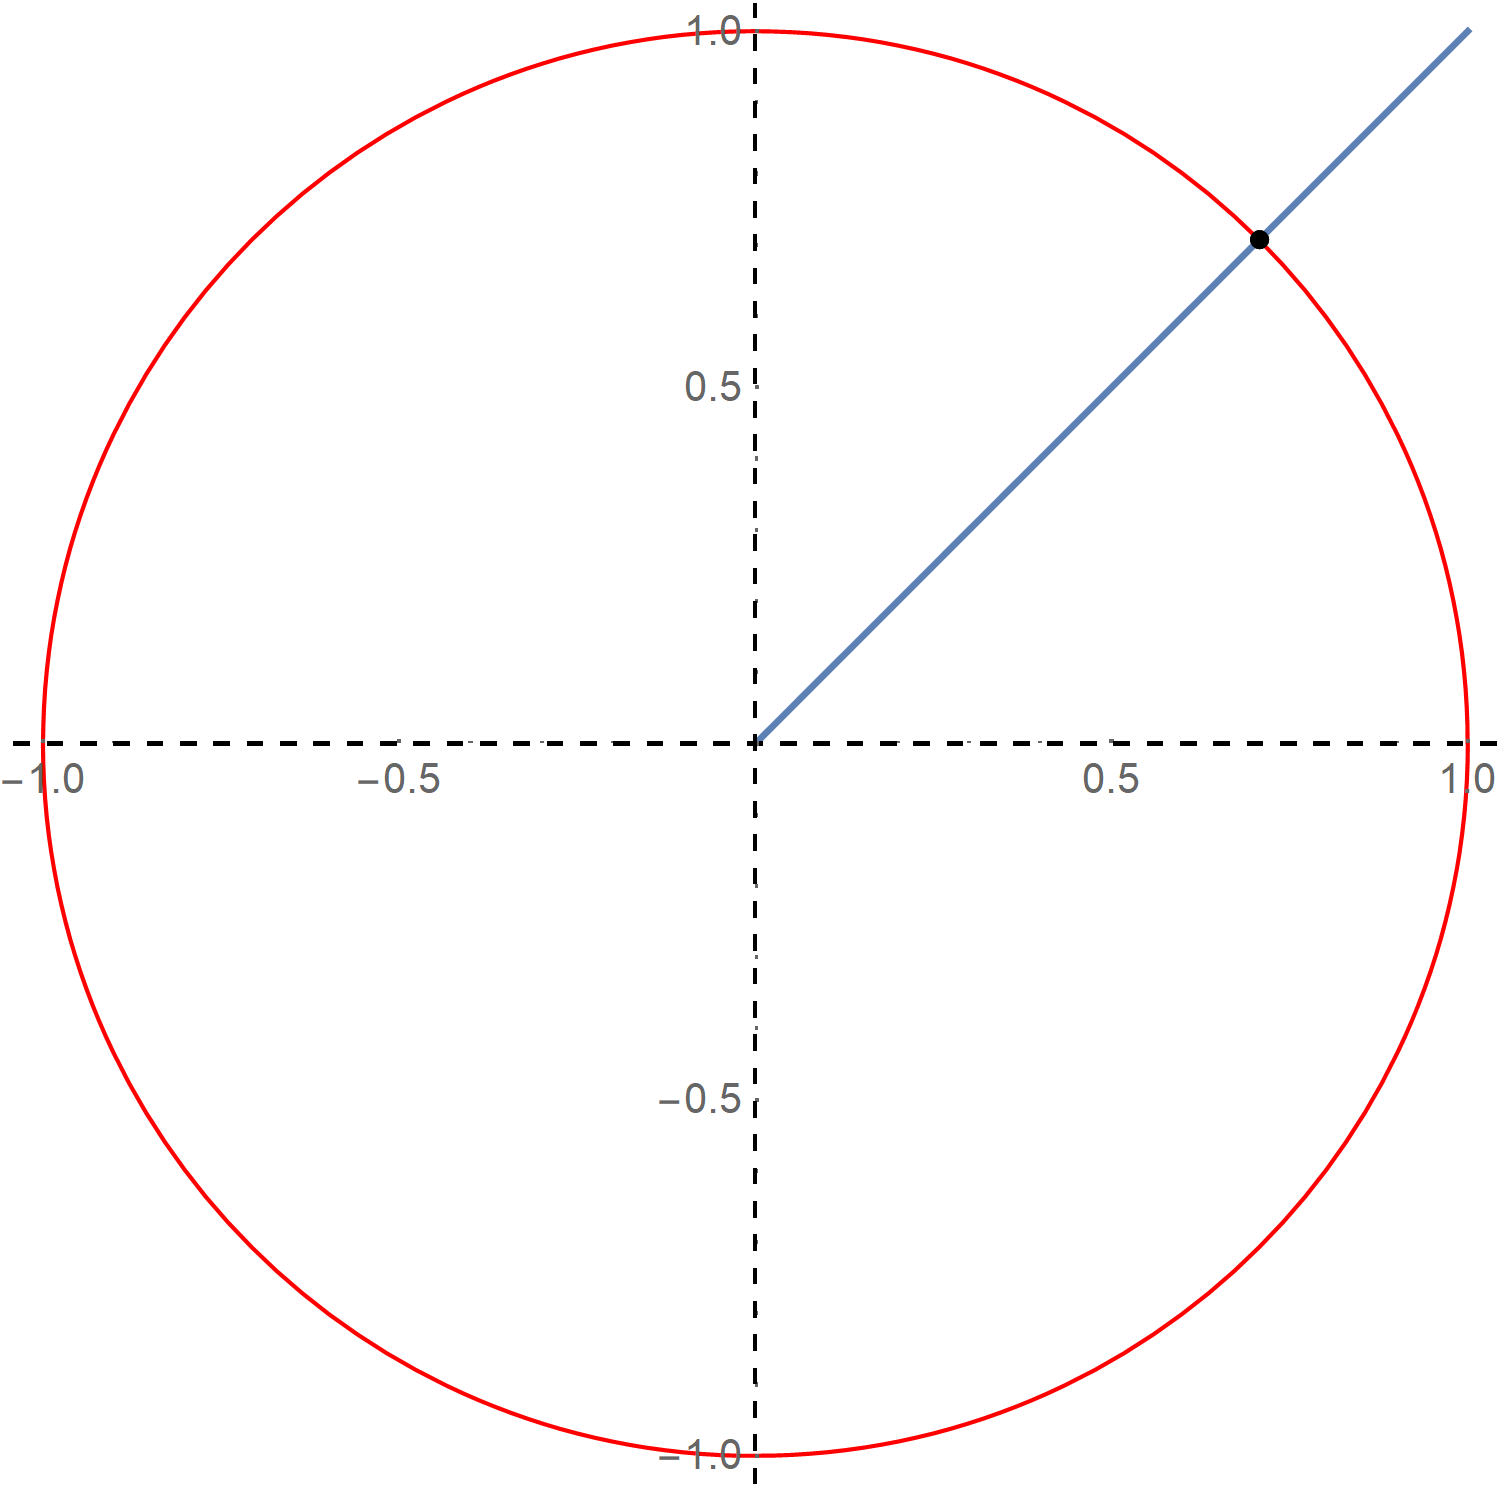
\includegraphics[trim = 0 0 0 0, clip, scale = 1]{Paper-Poster/CircleModuliSpace.png}
    \caption{Moduli Space of Lines in Plane}
\end{figure}
%In addition to finding a visual representation, we also wanted to determine the relationship between the planes. The quaternions are only one example of a Central Simple Algebra (CSA) and by generalizing our construction of the quaternions, we can study other 4D CSAs over \bR. 
}
\end{block}

\vskip2ex

\end{column}

\begin{column}{\sepwid}\end{column}			% empty spacer column

%---- COLUMN 2 ---------------------------------------------------------%
\begin{column}{\onecolwid}
%-------- BLOCK -------------------------------------------------------%
\begin{block}{Commutative Planes in the Quaternions}
\rmfamily{%


%The embeddings of \bC into \bH are determined by injective homomorphisms $\Psi : \bC \rightarrow \bH$ such that $\Psi|_{\bR}$ is the identity map. Here, $\Psi$ is completely determined by where it sends $i$, and since it is a homomorphism, we have the necessary condition that $\Psi(i)^2 = -1$. This condition is enough to determine the space of embeddings.

We started with an attempt to visualize all of the complex planes inside of \bH by representing them as points in a moduli space. We found that the oriented complex planes in \bH are naturally represented by points on a sphere, where each point represents the ``$i$'' of a different complex plane.
}

\begin{alertblock}{\textsf{Moduli Space of Planes in Quaternions}}
    \rmfamily{
        \begin{figure}
            \centering
            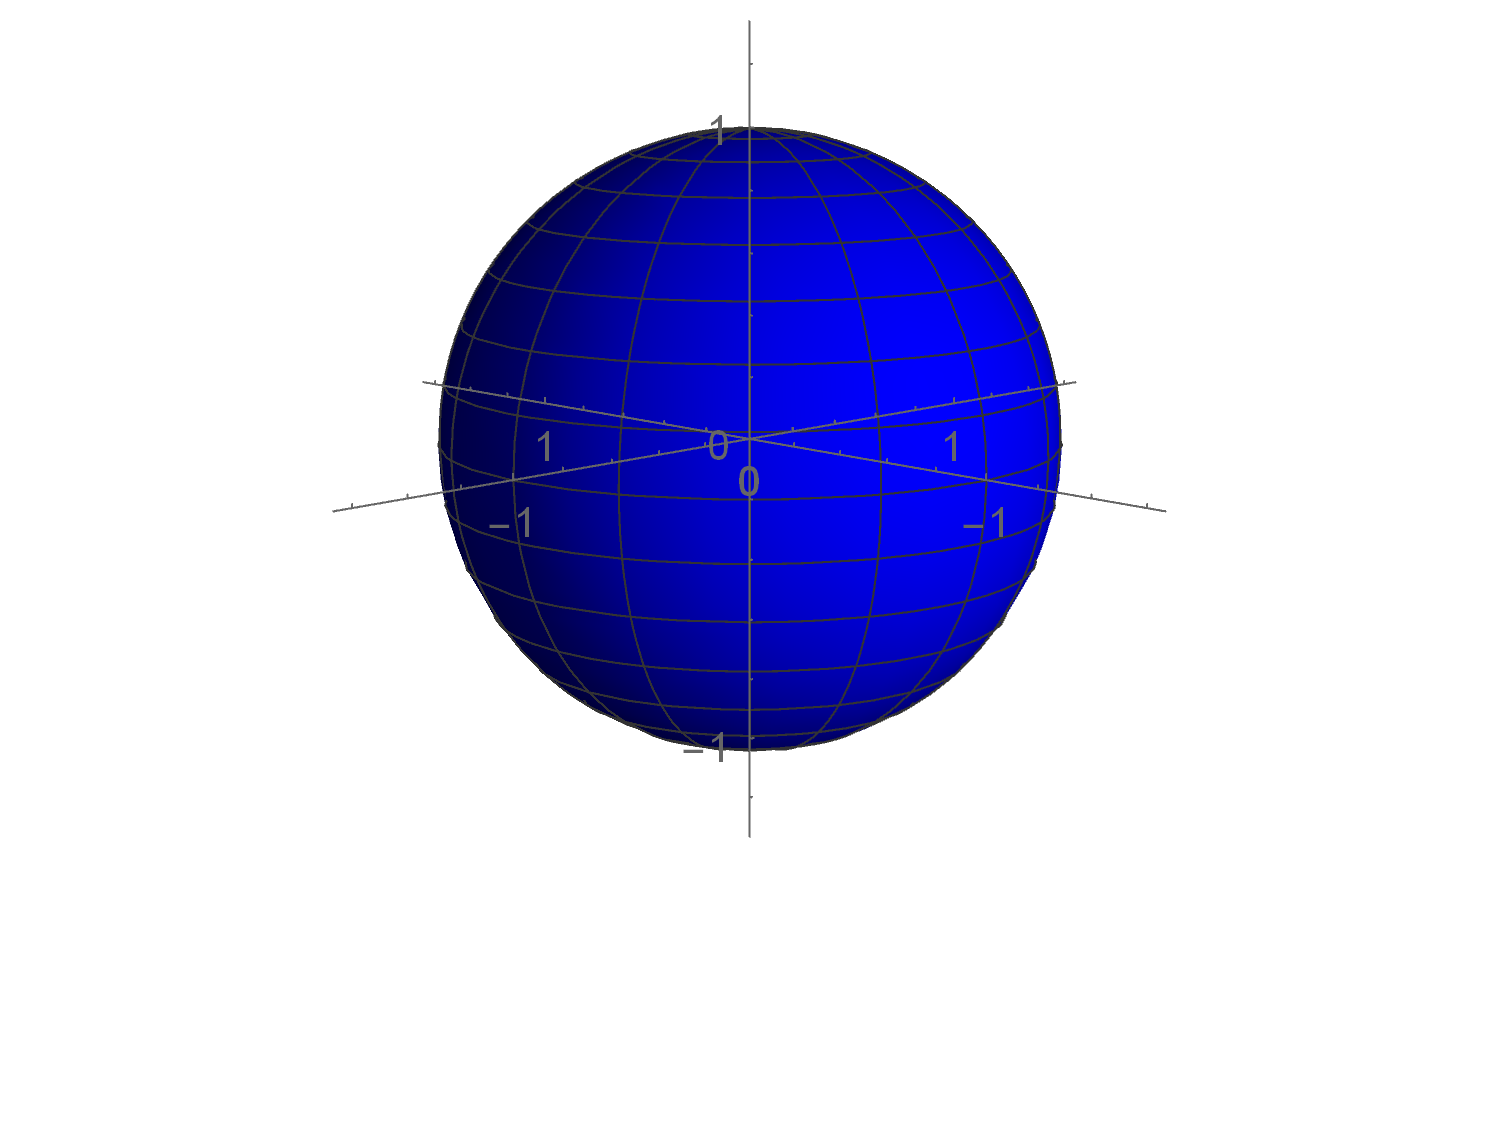
\includegraphics[trim = 75 65 75 0, clip, scale = 2.8]{Paper-Poster/QuatSphere.png}
            \caption{Moduli Space of \bC in \bH}
            \label{fig:QuatSphere}
        \end{figure}
    }
\end{alertblock}

Along with this visual representation, we found that these planes were shuffled amongst themselves by the inner automorphisms of \bH. All inner automorphisms of \bH can be represented as conjugation by an element of the 3-sphere $S^3$, which amazingly, is itself a (simply connected) subgroup of \bH. This is summarized by the short exact sequence:

\begin{equation*}
\begin{tikzcd}
1 \arrow{r} & \{\pm 1\} \arrow{r} & S^3 \arrow{r} & SO_3 \arrow{r} & 1
\end{tikzcd}
\end{equation*}
%In addition, this sphere represents all possible 2 dimensional commutative sub-algebras inside of \bH. They are the largest possible commutative sub-algebras of \bH and form a single conjugacy class under the action of $S^3$.
\end{block}


\begin{block}{Generalized Quaternions and Wedderburn}
\rmfamily{
We first characterized the planes in \bH, but the construction of \bH can be generalized. To study all CSAs over \bR, we introduce the generalized quaternions: 
}
\end{block}
\begin{alertblock}{Generalized Quaternions}
\rmfamily{
    Let $\mathbb{F}$ be a field and $a,b \in \mathbb{F}$
        \begin{align*}
            A_{a,b}(\mathbb{F}) &= \left\{t+xi+yj+zk: 
            \begin{aligned}
                & t, x, y, z \in \mathbb{F}, \\
                & i^2 = a, j^2 = b, \\
                & ij = -ji = k 
            \end{aligned}
            \right\}
        \end{align*}     
}                
\end{alertblock}

\rmfamily{
Wedderburn's theorem tells us that every CSA is either a division algebra or a matrix ring over a division algebra. We also have a set of isomorphisms between different generalized quaternions. We can then show that there are only two classes of 4D generalized quaternions over \bR, namely: $ A_{-1,-1}(\bR) &\simeq \bH$ and $A_{1,1}(\bR) &\simeq M_2(\bR)$. 
}


\end{column}

\begin{column}{\sepwid}\end{column}			% empty spacer column

%---- COLUMN 3 ---------------------------------------------------------%
\begin{column}{\onecolwid}
%-------- BLOCK -------------------------------------------------------%

\begin{block}{Commutative Planes in the 2x2 Matrices}
\rmfamily{%
%We now turn to the second isomorphism class of generalized quaternions over \bR. The ring of two by two real matrices: $M_2(\bR) \simeq A_{1,1}(\bR)$.
%As in the case of \bH, we are interested in the copies of planes inside of $M_2(\bR)$. However, unlike the standard quaternions, there ends up being more than one type of plane.
%In total, there are three different types of commutative planes inside of $M_2(\bR)$. There is the standard complex plane \bC, the split plane $\bR \times \bR$, and a third that we refer to as the nilpotent plane.
Any two linearly independent matrices in $M_2(\bR)$ span a plane, and just like in \bH, the plane may itself be a number system, this time under matrix multiplication.
As in \bH, we aim to construct a moduli space for these planes. However, we found more types of planes, not just \bC, but additionally the {\it split plane} $\bR\times\bR$, and a third, degenerate plane type, which we call the {\it nilpotent plane}.
\newline

We can construct individual moduli spaces for the three plane types based on their characteristic elements (square roots of -1, nontrivial idempotents, and nontrivial nilpotents, respectively).


\vskip2ex
\begin{figure}
    \centering
    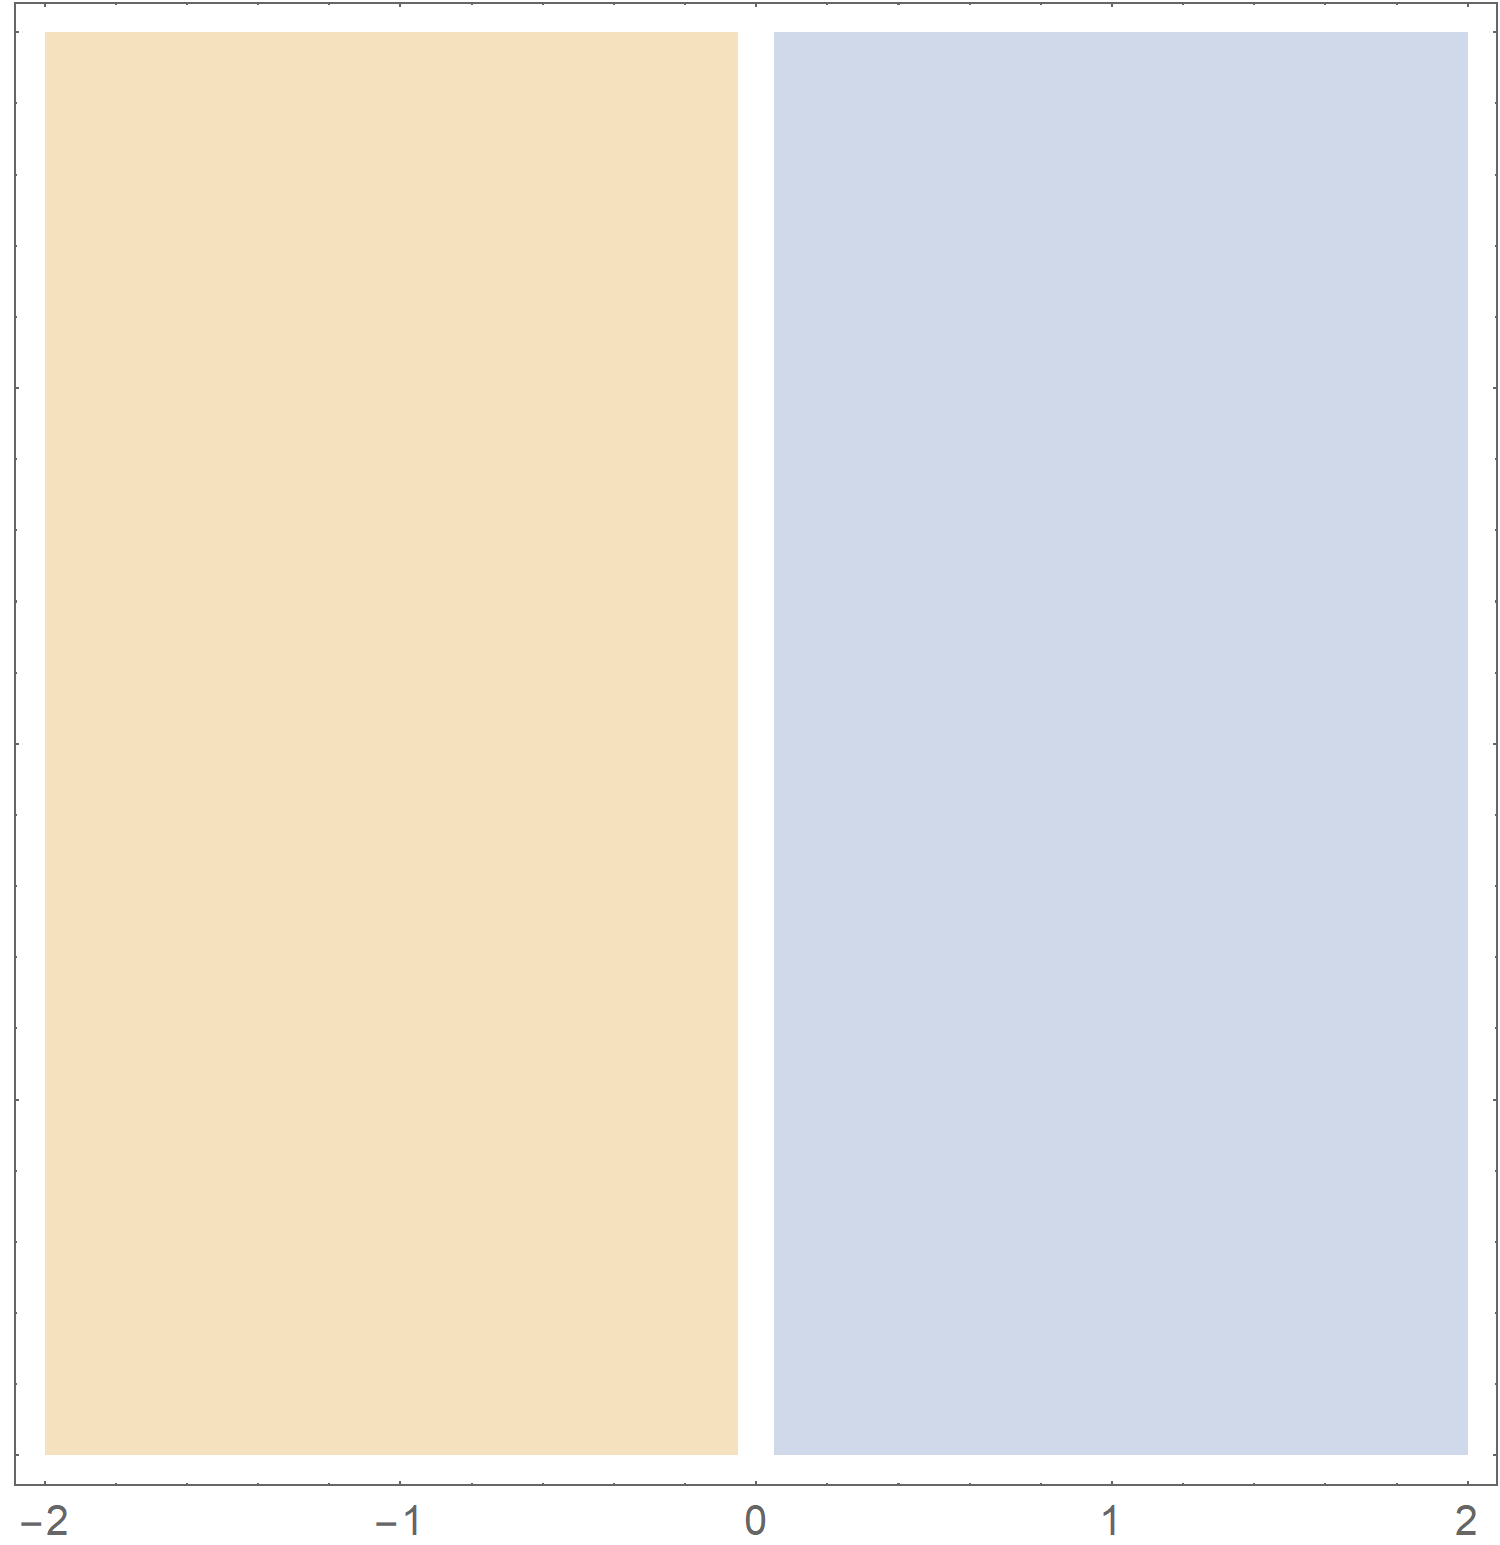
\includegraphics[trim = 0 0 0 0, clip, scale = 1]{Paper-Poster/SplitPlane.png}
    \caption{Moduli Space of \bC in $M_2(\bR)$}
\end{figure}
\vskip2ex

Pictured above is the moduli space of complex planes in $M_2(\bR)$. Each point not on the y-axis represent one such complex plane. The two halves represent two orbits under the (transitive) conjugation action of the simply connected group $SL_2(\bR)$.

\vskip2ex
\begin{figure}
    \centering
    \subfigure{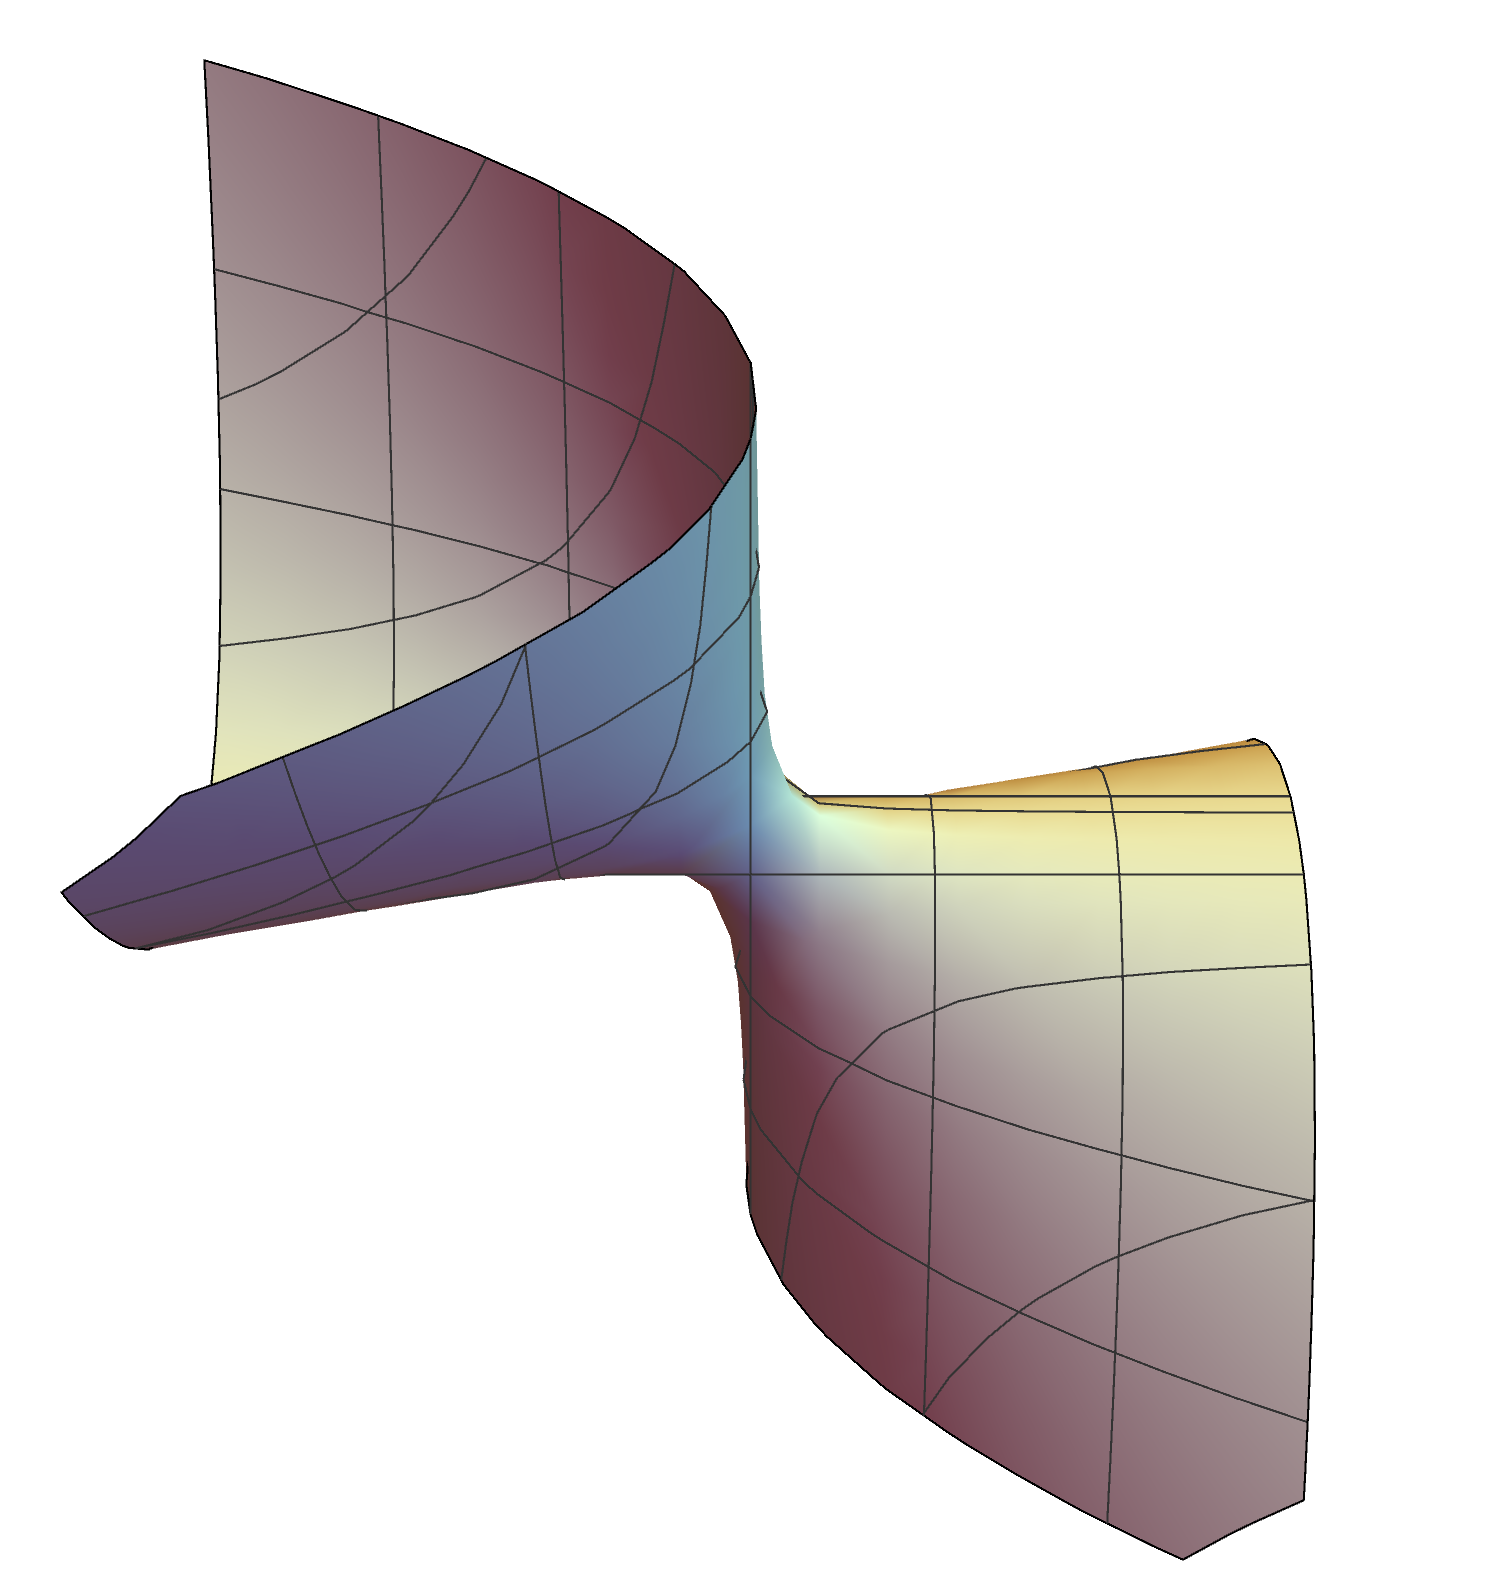
\includegraphics[]{Paper-Poster/RxR.png}}
    \hfill
    \subfigure{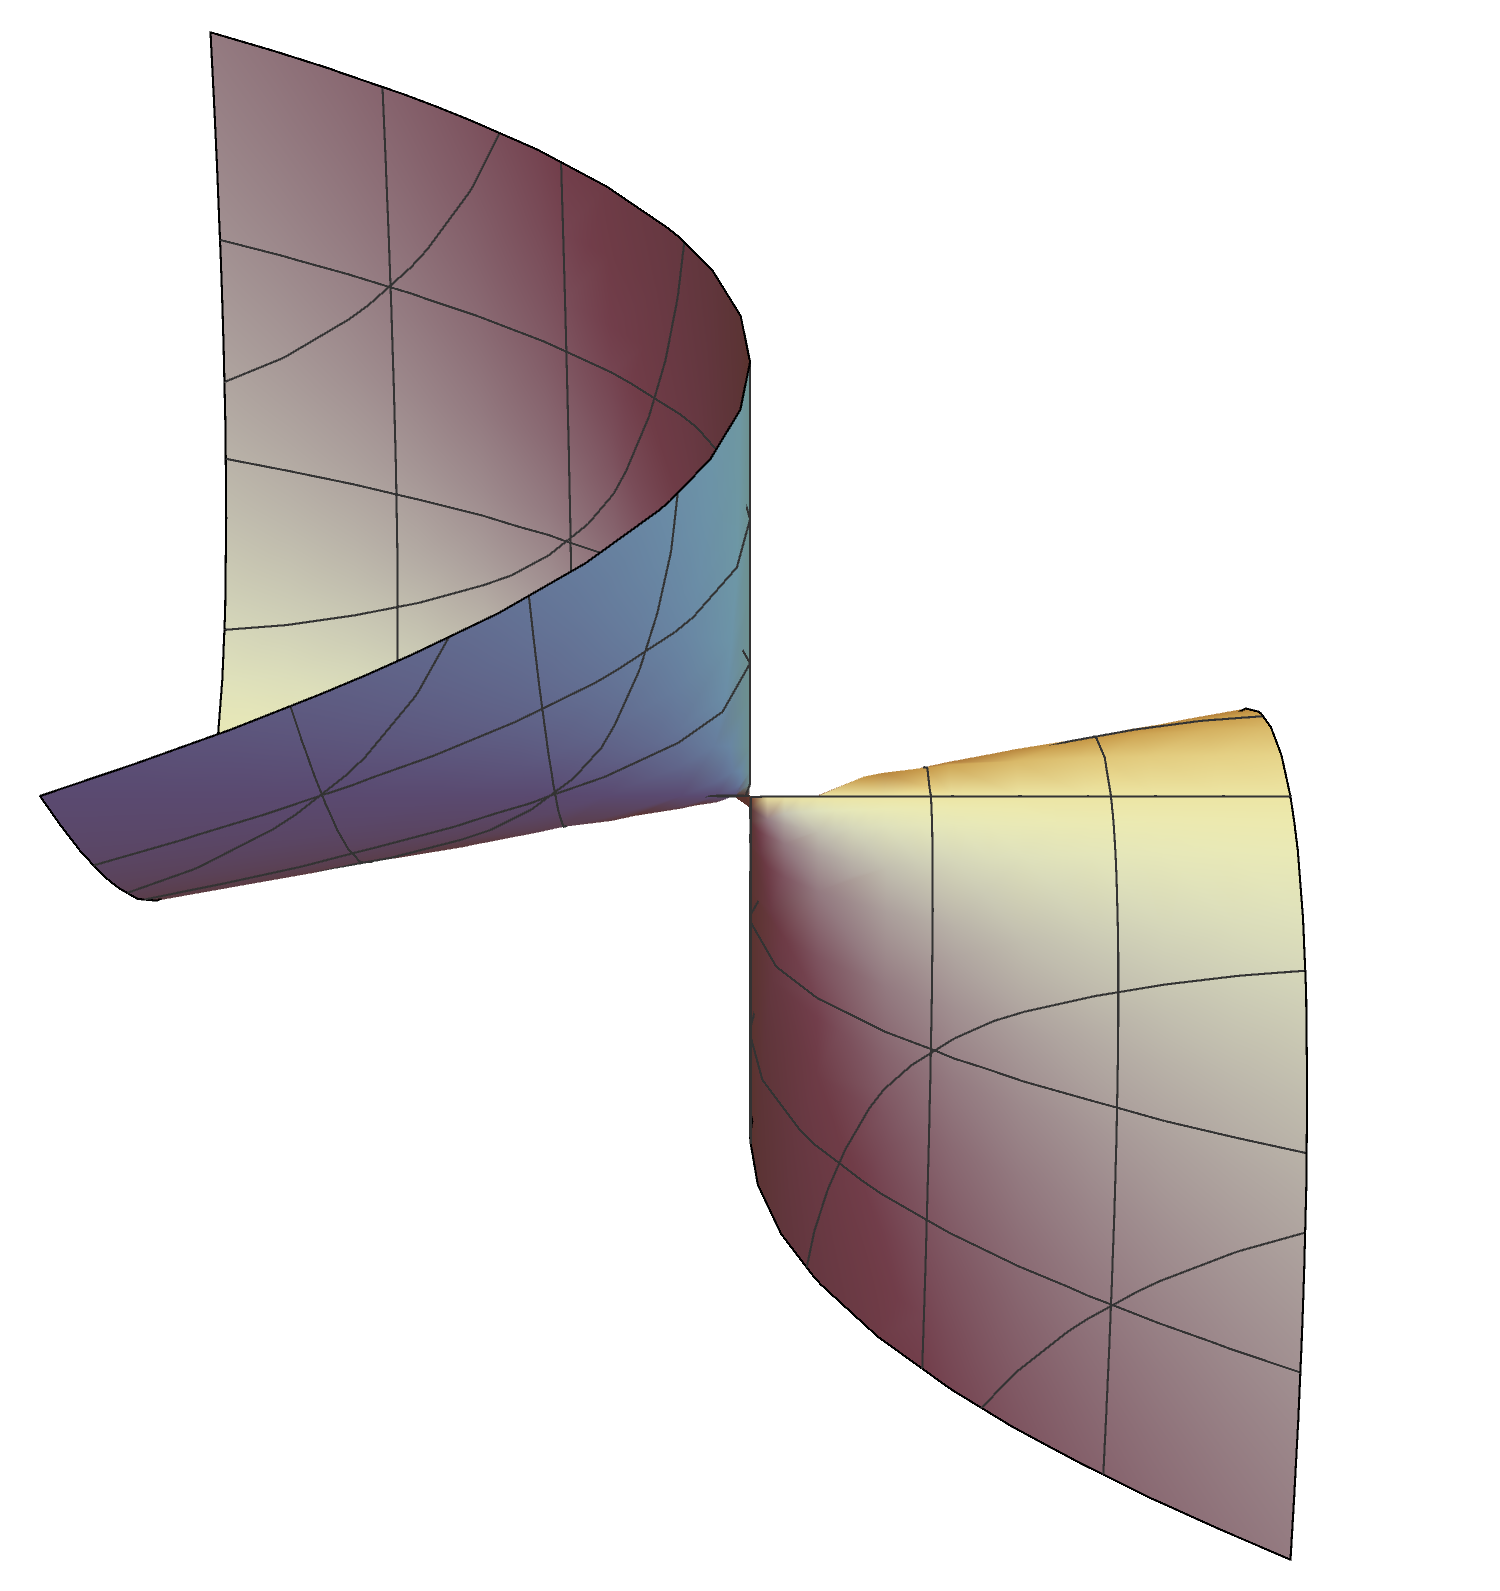
\includegraphics[]{Paper-Poster/Nilpotents.png}}
    \caption{Moduli Space of $\bR\times\bR$ (Left) and Nilpotents in $M_2(\bR)$ (Right)}
\end{figure}
\vskip2ex

Similar to the complex planes, the nilpotent planes form two orbits under the action of $SL_2(\bR)$. In contrast, the copies of $\bR\times\bR$ form a single orbit.
\newline

Finally, we combine these three moduli spaces into a single moduli space representing all three types of planes. This is summarized by a short exact sequence analogous to the one that appears for the quaternions:
%In doing so, we discovered a relationship between moduli space structure and the structure of the conjgucay classes of the plane types that require further exploration

%Mirroring the quaternions case, we can construct any one of these planes by first taking the multiplicative identity from the embedded real axis and then adjoining a unit length element from the orthogonal complement of the real axis to form a basis. This gives a sphere's worth of planes similar to the moduli space construction in \bH. We can then determine the type of plane that is created based on the point from the sphere chosen.
}
\begin{equation*}
    \begin{tikzcd}
        1 \arrow{r} & \{\pm 1\} \arrow{r} & SL_2(\bR) \arrow{r} & PSL_2(\bR) \arrow{r} & 1
    \end{tikzcd}
\end{equation*}

\vskip2ex

\end{block}


\vskip2ex

%-------- BLOCK -------------------------------------------------------%
\end{column}
%
\begin{column}{\sepwid}\end{column}			% empty spacer column
%

%---- COLUMN 4 ---------------------------------------------------------%
\begin{column}{\onecolwid}

\begin{alertblock}{Moduli Space of Planes in 2x2 Matrices}
    \begin{figure}
        \centering
        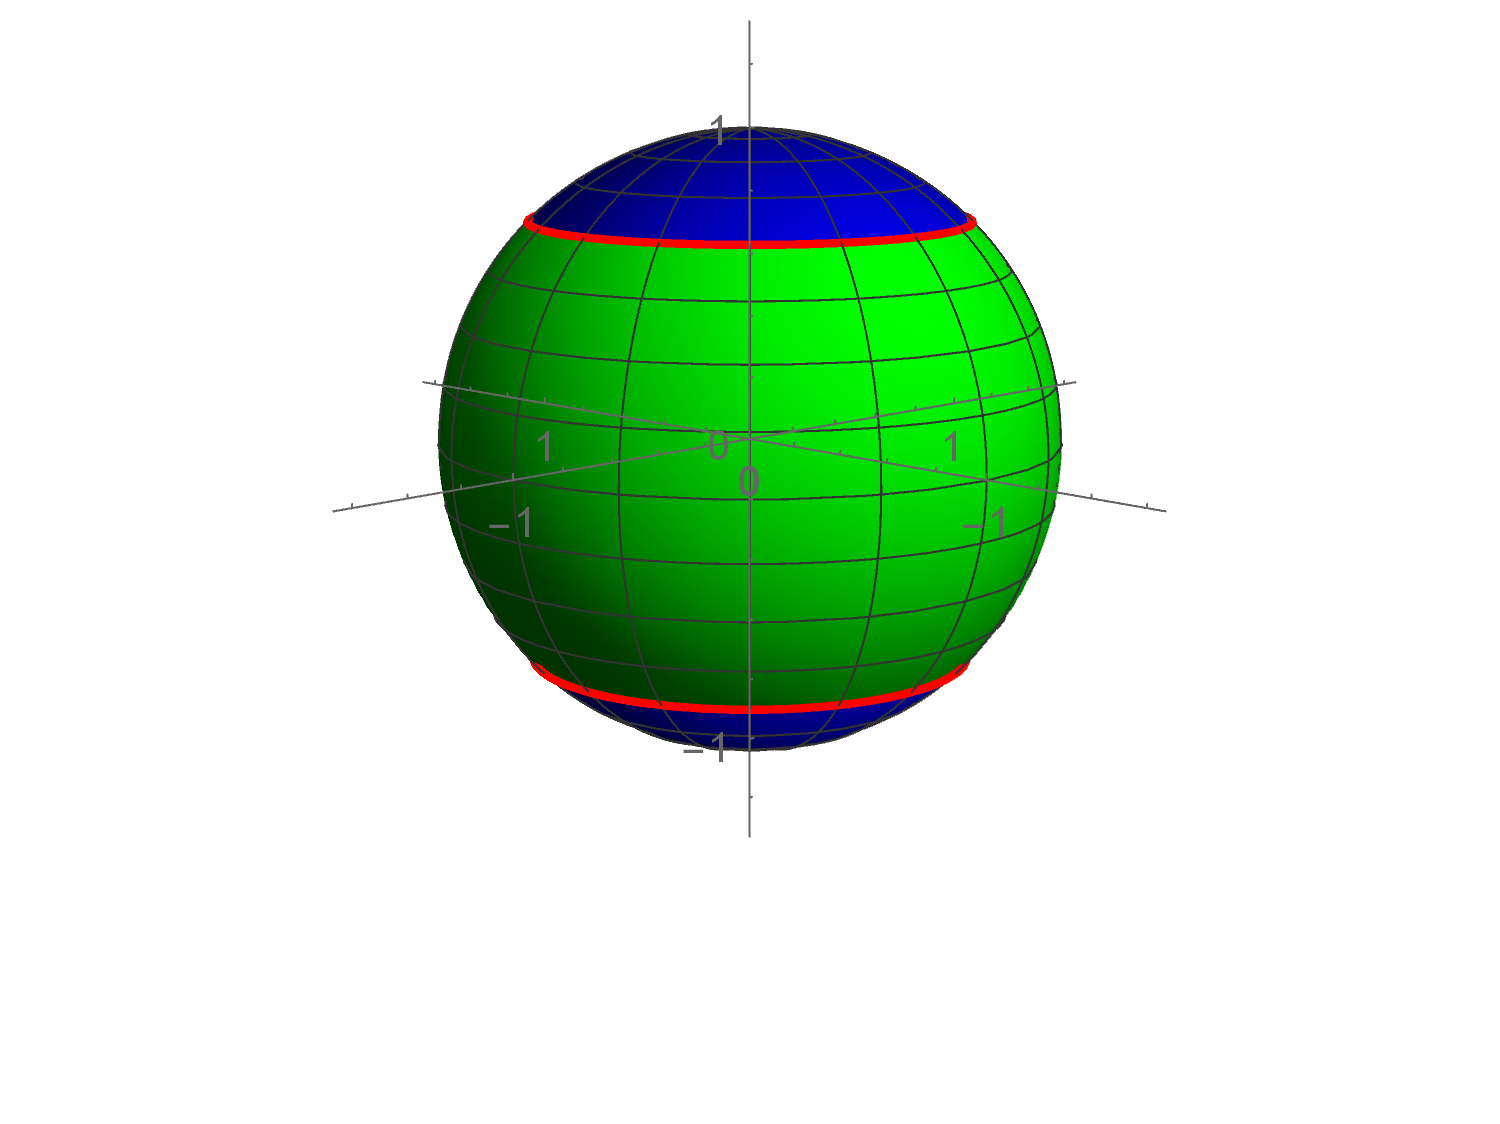
\includegraphics[trim = 75 65 75 0, clip, scale = 2.8]{Paper-Poster/MatricesSphere.png}
        \caption{Moduli Space of Planes inside $M_2(\bR)$}
    \end{figure}
\end{alertblock}

\rmfamily{
In the sphere moduli space above, each color corresponds to a different type of plane. Therefore this moduli space defines a {\it probability distribution} for the different types of planes inside of $M_2(\bR)$, based on the ratio of surface areas. That is, if we were to pick a plane at random, the probability that it would be \bC, $\bR\times\bR$, or nilpotent would be $1-\frac{1}{\sqrt{2}}$,$\frac{1}{\sqrt{2}}$, and 0 respectively.
}
\vskip2ex

%-------- BLOCK -------------------------------------------------------%
\begin{block}{Conclusions}
\rmfamily{%
 We determined that the set of all complex planes in \bH are naturally represented by the points on a sphere. We discovered 3 types of planes in $M_2(\bR)$, whose union is all of $M_2(\bR)$. As in \bH, we found that each plane is naturally represented by the points on a sphere, so that again the sphere is a moduli space for the planes of $M_2(\bR)$. The three plane types take up different areas on the sphere, and determines a probability distribution for the three plane types.
}
\end{block}

\vskip2ex

%-------- BLOCK -------------------------------------------------------%
\begin{block}{Further Work}
\rmfamily{%
\begin{enumerate}
    %\item Build out a notion of the probability distribution of the three plane types in $M_2(\bR)$ as well as generalized quaternions over finite fields.
    \item Give a constructive proof of Wedderburn's Theorem for the generalized quaternions over an arbitrary field.
    \item Investigate the structure of commutative subalgebras of generalized quaternions over \bQ, $\bQ_p$, and finite fields $\mathbb{F}_{p^n}$.
    \item Establish a unified theory for the structure of commutative subalgebras of the generalized quaternions over arbitrary fields.
\end{enumerate}

}
\end{block}
\vskip2ex

%-------- BLOCK -------------------------------------------------------%
\begin{block}{Acknowledgements}
\rmfamily{%
Special thanks to the Bill and Linda Frost Fund for support. This research was conducted by Frost Research Fellows under the Frost Undergraduate Research Award. 
}
\end{block}
\vskip2ex

\end{column}
\begin{column}{\sepwid}\end{column}			% empty spacer column
\end{columns}
\end{frame}
\end{document}

